\subsection{Non Programmable Privacy}

In addition to Zcash, there are other public blockchains facilitating private transactions, such as Monero \cite{website:Monero}, Dash \cite{website:Dash}, Grin \cite{website:Grin}, etc. However, these blockchains only support basic private asset transfers but lack programmability. As a result, their ecosystem development significantly trails Ethereum, which has become the largest public blockchain in the ecosystem due to its programmability. Nevertheless, Ethereum does not have privacy features.
To address this issue, some projects have started exploring ways to introduce privacy to Ethereum, such as the \textit{ZK-ZKRollup} application zk.money, developed by the Aztec team. Unfortunately, the zk.money product has been discontinued, primarily because its privacy features were limited to basic single transfer scenarios. Given the current surge in decentralized finance (DeFi) applications, asset transfers represent just one of the simplest financial scenarios. Consequently, the user base is limited, while maintenance costs continue to accumulate.

Therefore, some projects have begun to explore ways to introduce privacy to Ethereum, such as the \textit{ZK-ZKRollup} application \textit{zk.money} \cite{website:zk.money} developed by the \textit{Aztec} \cite{website:Aztec} team. However, the current \textit{zk.money} product has been discontinued, mainly because its privacy features only apply to simple single transfer scenarios. Given the current explosion of DeFi applications, asset transfer is only one of the simplest financial scenarios, and therefore the user base is limited, while the maintenance costs continue to accrue.
\begin{figure}[!ht]
    \centering
    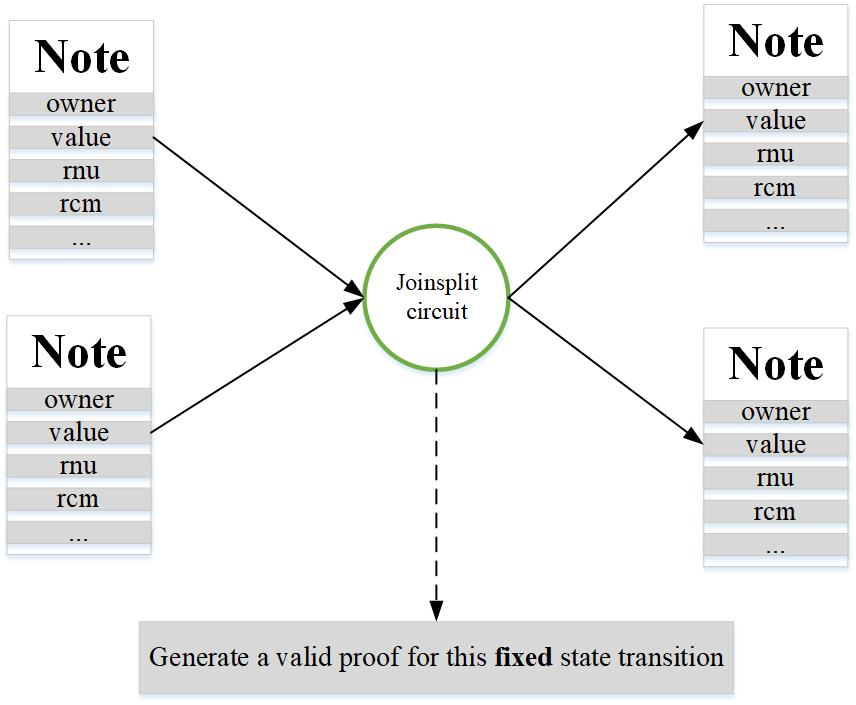
\includegraphics[width=0.4\textwidth]{Example of Non Programmable privacy.jpg}
    \caption{Example of Non Programmable Privacy}
    \label{fig:Example of Non Programmable Privacy}
\end{figure}

\figref{fig:Example of Non Programmable Privacy} shows the simple logic of non-programmable privacy. The value change logic corresponding to the input and output notes in Section \ref{section: sending-notes} are also fixed, generally in the form of ``$A + B = C + D$''. \textit{Manta Network} \cite{website:Manta-network} is a public blockchain that supports user-defined token privacy transfers, and the privacy transaction constraint circuits of all fungible tokens can be used to reuse the above logic.

A ZK-ZKRollup of a single-use case application, is similar to a corresponding ZKRollup of a single-use case application. If you want to use an asset in another application, you must bridge the asset through another protocol, which is generally a poor user experience. Therefore, just as ZKRollups need to transition to ZK(E)VMs, ZK-ZKRollup also needs to transition to ZK-ZKVMs (Appendix \ref{section: solidity-compatibility} explains how to get solidity compatibility).
